\documentclass[a4paper,fleqn]{cas-sc}
\usepackage[authoryear,longnamesfirst]{natbib}
\usepackage{amsmath,booktabs,xcolor}
\newcommand{\todo}[1]{{\color{red}[TODO: #1]}}
% Numbers: scripts/frl_analysis.py -> frl_analysis.json (Tables 1-2, Fig 3, robustness);
% scripts/frl_fig2.py -> fig2_cases.json (Fig 2); scripts/frl_fig1.py (Fig 1).
% Source: results/frl/minteval_v0_frl.csv.

\begin{document}
\let\WriteBookmarks\relax
\def\floatpagepagefraction{1}
\def\textpagefraction{.001}
\shorttitle{Silent implementation shortfall}
\shortauthors{S. Wang, Y. He and V.Y. Wang}

\title[mode = title]{Silent implementation shortfall: Do large language models execute the trading strategy they are asked to write?}

%% Author order for this paper to be agreed by the three authors.
%% arXiv:2610.16384 order is V.Y. Wang, S. Wang, Y. He.
\author[1]{Siyu Wang}[orcid=0009-0004-5071-3671]
\ead{24300680134@m.fudan.edu.cn}
\credit{Methodology, Formal analysis, Writing -- original draft}

\author[1]{Yuecheng He}[orcid=0000-0000-0000-0000]
\ead{yche24@m.fudan.edu.cn}
\credit{Methodology, Formal analysis, Writing -- original draft}

\author[1,2,3]{Varstern (Yifan) Wang}[orcid=0009-0002-7570-9148]
\cormark[1]
\ead{wag25528@gmail.com}
\credit{Conceptualization, Software, Data curation, Writing -- review \& editing}

\affiliation[1]{organization={Fudan University},
                city={Shanghai},
                country={China}}
\affiliation[2]{organization={Spearmint AI},
                country={China}}
\affiliation[3]{organization={NexusLumenLabs},
                country={China}}

\cortext[cor1]{Corresponding author.}

\begin{abstract}
Large language models (LLMs) are increasingly asked not only for market views but for the code that executes a trading strategy. We measure the implementation shortfall this creates: the gap between the strategy a trader describes and the strategy that actually runs. Using MintEval \citep{wang2026minteval}, in which reference strategies with known bar-by-bar behaviour are described in trader language and re-implemented by a model, we hold market data, frictions and the strategy itself fixed, so that any return difference is attributable to the implementation alone. Across four low-cost models the median absolute shortfall is 442--2{,}252 basis points of initial equity, and 37--81\% of implementations run without error yet diverge from the intended behaviour. The shortfall is a dispersion rather than a bias: for the two strongest low-cost models the mean signed shortfall is within 60 bp of zero while the mean absolute shortfall exceeds 1{,}100 bp. It is state-dependent: it rises with how long the strategy must remember its risk state, by about 180 bp per tenfold increase in state span, and the rise is steeper when markets are volatile. A frontier model reduces but does not remove the problem (27.5\% silent divergence). Because the failure survives compilation, backtesting and semantic review, it is a model risk that standard pre-deployment checks do not cover.
\end{abstract}

\begin{highlights}
\item We measure the gap between the strategy a trader describes and the one an LLM codes.
\item Strategy, data and frictions are fixed, so the gap isolates implementation error.
\item Median absolute shortfall is 442--2{,}252 bp; most failures run without error.
\item Shortfall is state-dependent: it grows with state span, more so when volatile.
\item The failure is invisible to compilation, backtesting and code review.
\end{highlights}

\begin{keywords}
Large language models \sep Algorithmic trading \sep Implementation shortfall \sep Model risk \sep Code generation
\end{keywords}

\maketitle

%% ------------------------------------------------------------------
\section{Introduction}

Research on LLMs in investment management has focused on the model as a producer of views: stock selection \citep{ko2024,pelster2024}, sentiment \citep{kirtac2024}, factor generation \citep{cheng2024}, return prediction \citep{lopezlira2023}, and the behaviour of an LLM acting as a quantitative manager \citep{kim2023}. In all of these the LLM supplies a signal and a human or a conventional system executes it.

A second use is growing quietly in practice: the LLM writes the code. A trader describes entry rules, position sizing and a stop in ordinary language, and the model returns a strategy that is backtested and, increasingly, connected to an execution venue. \citet{perold1988} defined implementation shortfall as the difference between a paper portfolio and the portfolio actually realised. LLM-written code introduces a component of this shortfall that did not exist before: the difference between the strategy the trader intended and the program that runs. The component is silent. The code compiles, the backtest completes and an equity curve appears; nothing signals that a breakeven stop never moves or that a cooldown resets every bar. Trading code errors are not hypothetical costs \citep{sec2013knight}, and backtests are already a fragile basis for decisions \citep{bailey2016}.

We ask two questions. (1) When an LLM implements a strategy from a natural-language instruction, how large is the shortfall relative to the intended strategy, and is it a bias or a dispersion? (2) Is the shortfall state-dependent: does it grow with the persistence of the strategy's risk logic and with market volatility, the conditions under which risk controls matter most?

We answer them with MintEval \citep{wang2026minteval}, a benchmark in which reference strategies are generated programmatically, described in either colloquial or indirectly-interpreted trader language, and re-implemented by the model under test. Reference and generated programs run on identical data with identical frictions. Because the strategy is given, alpha is differenced away and the return gap isolates implementation. We find a median absolute shortfall of 442 bp for the best low-cost model and 2{,}252 bp for the weakest. The shortfall does not systematically cost money: for GPT-5.4-mini and Claude Haiku the mean signed shortfall is statistically indistinguishable from zero, so the cost is dispersion around the intended outcome, which no scalar adjustment can remove. It grows with state span, by 176 bp per decade of $\tau_{\max}$ with block fixed effects and controls, and volatility steepens that gradient. A frontier model cuts the shortfall sharply but still diverges silently on 27.5\% of tasks.

Look-ahead and leakage deserve a word, since they are the usual concern when LLMs touch financial data \citep{glasserman2024}. Neither applies here. The backtest engine exposes only bars up to the current one and raises an error on any attempt to read ahead, so a generated program cannot leak future data into its equity curve. The tasks themselves are assembled from a combinatorial space at build time; neither the instructions nor the reference programs exist on the web, so they cannot be in any model's training data.

%% ------------------------------------------------------------------
\section{Experimental design}

\subsection{Benchmark}

We use MintEval v0 \citep{wang2026minteval}: 800 tasks on BTCUSDT 15-minute bars, 1 January 2022 to 31 December 2023, with taker fees of 5 bp and slippage of 1 bp per fill. Each reference strategy combines one signal, a filter, a sizing rule and one to three risk layers drawn from a library of 20 blocks; hard combinations include moving stop boxes, scaling out, pyramiding and risk layers that read each other's state. Two properties of each strategy are recorded. $K$ is its description length in the generator's grammar. $\tau_{\max}$ is the longest span, in bars, between a write to and a read from any state variable during the reference backtest, measured by instrumenting execution; it captures how long the strategy must remember something. Tasks are stratified jointly on $\tau_{\max}$ quintile and reference return, giving median reference returns of $-0.37$, $-0.37$, $-0.37$, $-0.34$ and $-0.34$ across quintiles, and $\mathrm{corr}(\log\tau_{\max},K)=-0.03$. Each program is back-translated into a 40--120 word desk message with at least three slang expressions; 780 of 800 messages are verified by an independent reader to identify the intended strategy. Construction details are in \citet{wang2026minteval}. Figure~\ref{fig:pipeline} places the quantity we measure in the trading pipeline.

\begin{figure}
\centering
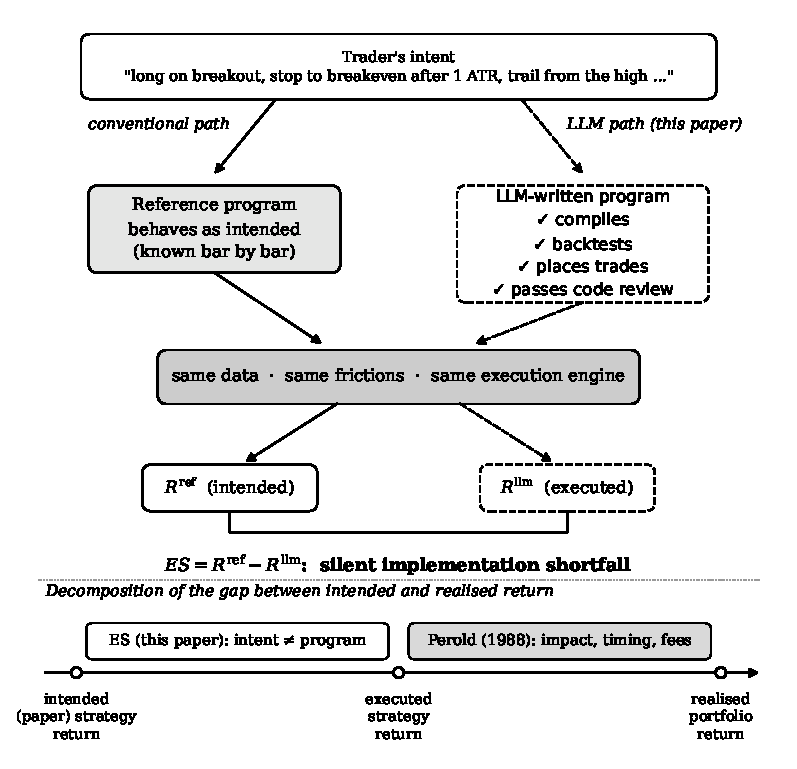
\includegraphics[width=.8\textwidth]{figs/fig1_pipeline.pdf}
\caption{Where LLM-written code enters the trading pipeline, and the shortfall it introduces. A trader's intent is implemented either by a reference program known to behave as intended or by a program written by an LLM from the same natural-language description. The LLM program compiles, backtests, trades and passes code review, yet may not be the strategy that was described. Both programs are executed on identical data with identical frictions, so the return gap $ES$ isolates implementation error. It sits before the components of implementation shortfall identified by \citet{perold1988}, which arise only after the executed strategy is fixed.}
\label{fig:pipeline}
\end{figure}

\subsection{Models}

Four low-cost models are evaluated on all 800 tasks: GPT-5.4-mini, Claude Haiku, and Qwen2.5-Coder 32B and 7B, at temperature 0 with one sample per task. Our main results use the \emph{open} setting, in which the model receives only the instruction and an interface document; a \emph{closed} setting that also lists the available blocks is used in Section~\ref{sec:understanding}. Claude Opus 5.5 is evaluated on a 200-task subset stratified identically.

\subsection{Measuring shortfall}

For task $s$ and model $m$ let $R^{\mathrm{ref}}_s$ be the reference return and $R^{\mathrm{llm}}_{s,m}$ the return of the generated program on the same data. We define
\begin{equation}
ES_{s,m} = R^{\mathrm{ref}}_s - R^{\mathrm{llm}}_{s,m}, \qquad |ES_{s,m}|,
\end{equation}
both in basis points of initial equity. The signed measure answers whether implementation error systematically hurts; the absolute measure, which we treat as primary, answers how far the executed strategy is from the intended one. We winsorise at the 1st and 99th percentiles within each model. As a behavioural companion we report ActionMatch, the share of active bars on which the two programs hold the same quantised position, and call a run a \emph{silent failure} if it compiles but has ActionMatch below 0.9. Runs that fail to compile are excluded from $|ES|$ and reported separately; Section~\ref{sec:robust} treats them as the maximum loss.

\subsection{Identification and specification}

$\tau_{\max}$ is fixed by the generator before any model is run, so it cannot respond to a model's output, and stratification makes it orthogonal to how profitable the reference strategy is. We estimate
\begin{equation}
|ES_{s,m}| = \alpha + \beta_1 \log\tau_{s} + \beta_2 \sigma_{s} + \beta_3 \,\log\tau_{s}\times\sigma_{s} + \gamma' X_{s} + \mu_m + \eta_{b(s)} + \varepsilon_{s,m},
\label{eq:main}
\end{equation}
where $\log\tau_s$ is $\log_{10}\tau_{\max}$ centred on its task mean, $\sigma_s$ is the annualised realised volatility of BTCUSDT over the bars on which the reference strategy holds a position, standardised across tasks, $X_s$ contains $K$, log trade count, McCabe complexity and reference return, $\mu_m$ are model fixed effects and $\eta_{b(s)}$ are fixed effects for the signal block and an indicator for each risk block. Standard errors are clustered by task. $\beta_1$ is therefore the change in $|ES|$ per decade of $\tau_{\max}$ at average volatility and $\beta_2$ the change per standard deviation of volatility at average $\tau_{\max}$. $\beta_1>0$ says shortfall grows with state persistence; $\beta_3>0$ says volatility amplifies the cost of mis-implemented stateful logic.

%% ------------------------------------------------------------------
\section{Results}

\subsection{Magnitude}

Table~\ref{tab:main} reports the shortfall by model. The best low-cost model compiles 95.5\% of its programs but reproduces the intended behaviour on only 54.4\% of active bars, with a median $|ES|$ of 442 bp; 72.9\% of all its tasks are silent failures. The weakest model compiles 37.4\% and has a median $|ES|$ of 2{,}252 bp. Compilation is not the binding constraint for the two closed-source models: most of their failures run to completion.

\begin{table}[width=\linewidth,cols=7,pos=t]
\caption{Implementation shortfall by model, open setting, 800 tasks. $|ES|$, $ES$ and ActionMatch are over compiled runs; mean $ES$ is winsorised 1/99 within model, with its $t$-statistic in parentheses. Exact is the share of tasks reproduced on every active bar; Silent is the share of all tasks that compile with ActionMatch $<0.9$.}
\label{tab:main}
\begin{tabular*}{\tblwidth}{@{} LCCCCCC@{} }
\toprule
Model & Compile & Median $|ES|$ (bp) & Mean $ES$ (bp) & ActionMatch & Exact & Silent \\
\midrule
GPT-5.4-mini      & 0.955 & 442     & $-55$ ($-0.82$)       & 0.544 & 0.087 & 0.729 \\
Claude Haiku      & 0.948 & 752     & $-45$ ($-0.51$)       & 0.400 & 0.040 & 0.806 \\
Qwen2.5-Coder 32B & 0.601 & 1{,}646 & $-345$ ($-2.29$)      & 0.172 & 0.006 & 0.586 \\
Qwen2.5-Coder 7B  & 0.374 & 2{,}252 & $-1{,}059$ ($-4.60$)  & 0.081 & 0.001 & 0.372 \\
\midrule
Claude Opus 5.5 (200 tasks) & 1.000 & 0 & $-44$ ($-0.97$) & 0.889 & 0.575 & 0.275 \\
\bottomrule
\end{tabular*}
\end{table}

Figure~\ref{fig:example} shows what a silent failure looks like. In each panel the two programs hold identical positions and earn identical returns until the first bar on which the mis-implemented rule binds. In panel~(a) GPT-5.4-mini writes a breakeven stop whose trigger reads an entry price that is never stored, so the trigger compares the close with itself and the stop is never set; the reference exits at its entry price and the model rides the subsequent decline, falling 261 bp behind within the plotted 300 bars. In panel~(b) GPT-5.4-mini measures the breakout box over a window that includes the current bar, so the close can never exceed the box top and the program never trades. In panel~(c) Claude Opus 5.5 applies the four-hour trend filter to the opposite-signal exit as well as to the entry; the reference covers its short when RSI crosses back above 25, while the model holds it for a further 1{,}449 bars. Panel~(b) also shows why the shortfall is a dispersion: the trades the model fails to take lose money, so here the error happens to help.

\begin{figure}
\centering
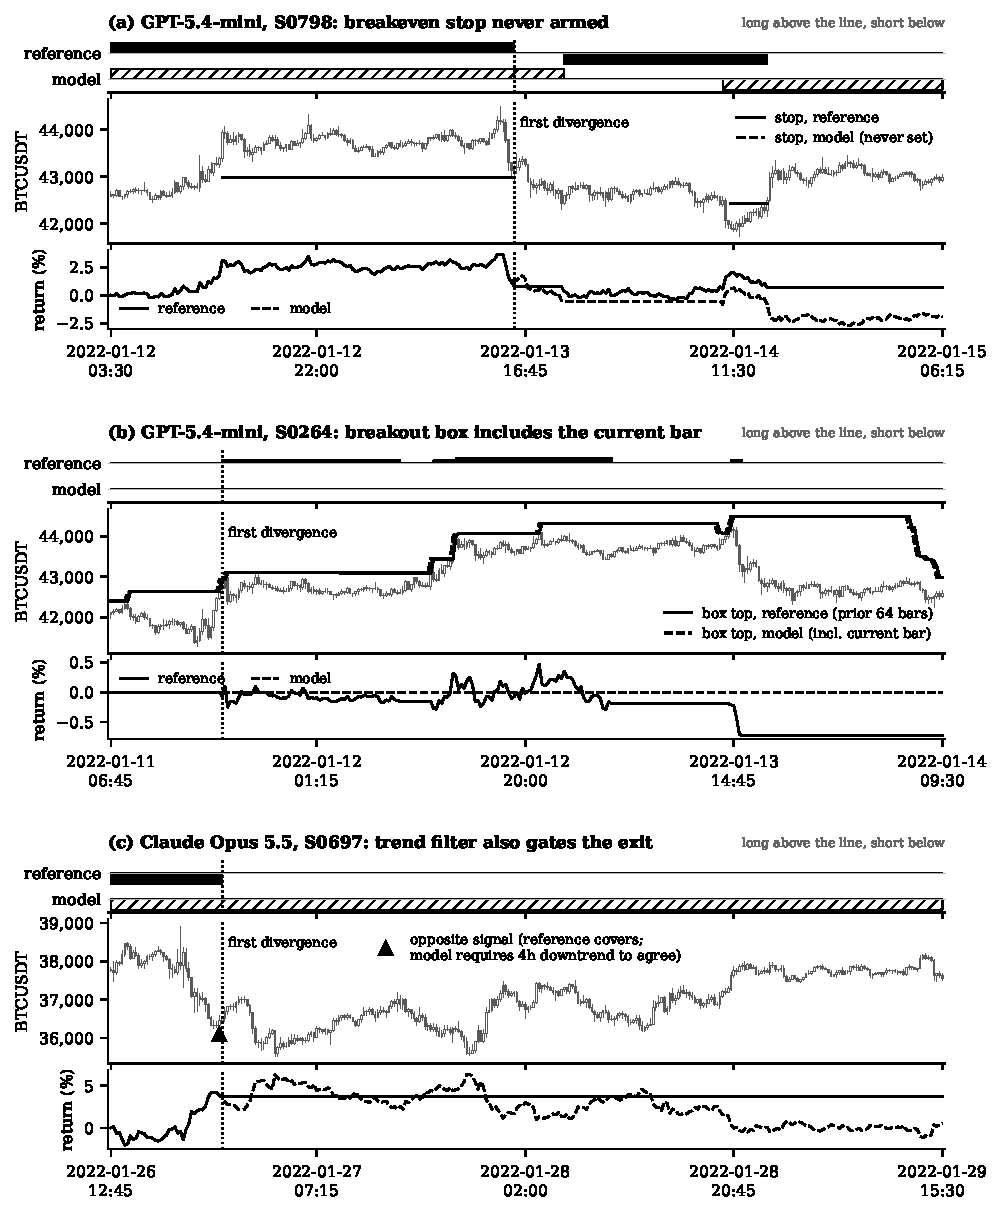
\includegraphics[width=\textwidth]{figs/fig2_examples.pdf}
\caption{Three silent failures. In each panel, top: position held by the reference program (solid) and the model's implementation (hatched), long above and short below the lane line. Middle: BTCUSDT 15-minute candles with the level each program is using. Bottom: cumulative return from the start of the window, reference (solid) and model (dashed). The curves coincide until the dotted bar, on which the mis-implemented rule first binds. (a) GPT-5.4-mini: the breakeven stop is never set because the entry price is never stored, so the drawdown it was meant to avoid is realised. (b) GPT-5.4-mini: the breakout box includes the current bar, so the close never breaks it and no position is ever opened. (c) Claude Opus 5.5: the trend filter is applied to the exit, so the opposite signal (triangle) on which the reference covers is ignored.}
\label{fig:example}
\end{figure}

\subsection{Bias or dispersion}

Implementation error does not systematically destroy value. For GPT-5.4-mini and Claude Haiku the mean signed shortfall is $-55$ and $-45$ bp, with $t$-statistics of $-0.82$ and $-0.51$, and the generated program beats the reference on 45\% and 46\% of compiled tasks and trails it on 46\% and 50\%; yet the mean absolute shortfall is 1{,}109 and 1{,}547 bp and the standard deviation of $ES$ is 1{,}870 and 2{,}433 bp. The same holds for Claude Opus 5.5 ($-44$ bp, $t=-0.97$). Only the two Qwen models have a significant mean, and it is negative ($-345$ and $-1{,}059$ bp): their broken programs trade less, often not at all (the median compiled Qwen2.5-Coder 7B program returns exactly zero), and with 15-minute frictions trading less loses less. The shortfall is therefore a dispersion around the intended outcome. For a risk manager this is the more troubling case: a bias could be corrected by a scalar haircut, whereas a dispersion means the executed strategy's return is a noisy and unpredictable transformation of the authorised one.

\subsection{Not an artefact of unprofitable references}

Reference strategies lose money after costs: the full-set median return is $-35.1\%$. This reflects 15-minute trading with 6 bp of frictions per fill (12 bp per round trip) rather than negative edge. With fees and slippage set to zero the median is $-0.6\%$ and 47.8\% of references are profitable. Losing references are, if anything, slightly easier to match, so they do not inflate the shortfall, and the state-span effect below is unchanged when reference return is controlled (Table~\ref{tab:reg}, column 4) or when the zero-cost reference return is added (Section~\ref{sec:robust}). Shortfall is therefore not a by-product of testing bad strategies; the same implementation errors would attach to profitable ones.

\subsection{State dependence}

Figure~\ref{fig:tau} plots median $|ES|$ by $\tau_{\max}$ quintile. For the two models whose programs mostly compile and partly work, the gradient is monotone or nearly so: GPT-5.4-mini rises from 186 bp in the first quintile to 897 bp in the fifth, and Claude Haiku from 359 bp to 1{,}198 bp. The Qwen models show no clear pattern; their compiled programs match the reference on fewer than a quarter of active bars in every quintile, so there is little correct behaviour left for state span to erode. Claude Opus 5.5 has a median $|ES|$ of at most 12 bp in every quintile, because it reproduces most tasks exactly. Table~\ref{tab:reg} estimates equation~\eqref{eq:main}. State span alone has a coefficient of 216 bp per decade ($t=2.91$, column 1), essentially unchanged when volatility is added (column 2). Volatility has an independent effect of 124 bp per standard deviation, and the interaction is positive (160 bp, $t=2.32$, column 3): longer-memory logic is costlier to get wrong in volatile markets. With controls and block fixed effects (column 4) the state-span coefficient is 176 bp ($t=1.70$, $p=0.09$), the volatility coefficient 154 bp ($t=2.61$) and the interaction 137 bp ($t=2.15$); estimates are similar for the low-cost models alone (column 5). For Claude Opus 5.5 alone (column 6) no coefficient is significant. For reference, the same gradient is present in behaviour: in \citet{wang2026minteval} ActionMatch falls by 0.065 (s.e.\ 0.013) per decade of $\tau_{\max}$ pooling the four low-cost models, and by 0.033 ($p=0.049$) once block fixed effects, McCabe complexity and trade count are controlled.

\begin{figure}
\centering
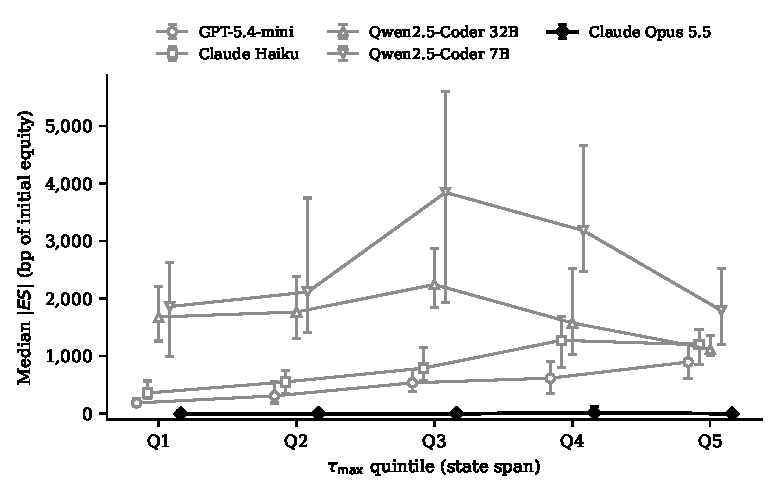
\includegraphics[width=.8\textwidth]{figs/fig3_tau.pdf}
\caption{Median absolute implementation shortfall by $\tau_{\max}$ quintile, compiled runs, with 95\% bootstrap intervals. Low-cost models (grey, open markers) and Claude Opus 5.5 (black).}
\label{fig:tau}
\end{figure}

\begin{table}[width=\linewidth,cols=7,pos=t]
\caption{Absolute implementation shortfall (bp, winsorised 1/99 within model) on state span and volatility, compiled runs, open setting. Columns (1)--(4) pool the four low-cost models (800 tasks each) and Claude Opus 5.5 (200 tasks). $\log\tau_{\max}$ is $\log_{10}$, centred; volatility is standardised. Controls are $K$, log trade count, McCabe complexity and reference return; block FE are signal-block fixed effects and risk-block indicators. Task-clustered $t$-statistics in parentheses.}
\label{tab:reg}
\begin{tabular*}{\tblwidth}{@{} LCCCCCC@{} }
\toprule
 & (1) & (2) & (3) & (4) & (5) Low-cost & (6) Opus \\
\midrule
$\log\tau_{\max}$               & 216.0  & 219.6  & 172.8  & 176.1  & 196.0  & $-236.0$ \\
                                & (2.91) & (2.94) & (2.31) & (1.70) & (1.77) & ($-1.67$) \\
Volatility $\sigma$             &        & 124.1  & 166.1  & 153.9  & 161.7  & 47.8 \\
                                &        & (2.82) & (3.38) & (2.61) & (2.58) & (0.67) \\
$\log\tau_{\max}\times\sigma$   &        &        & 160.2  & 137.2  & 139.8  & 100.2 \\
                                &        &        & (2.32) & (2.15) & (2.07) & (1.39) \\
\midrule
Controls          & No & No & No & Yes & Yes & Yes \\
Block FE          & No & No & No & Yes & Yes & Yes \\
Model FE          & Yes & Yes & Yes & Yes & Yes & -- \\
Observations      & 2{,}502 & 2{,}502 & 2{,}502 & 2{,}502 & 2{,}302 & 200 \\
Adjusted $R^2$    & 0.143 & 0.147 & 0.149 & 0.257 & 0.232 & 0.096 \\
\bottomrule
\end{tabular*}
\end{table}

Economically, a one-decade increase in $\tau_{\max}$ raises $|ES|$ by 176 bp at average volatility and by 313 bp at one standard deviation above it; a one-standard-deviation increase in volatility raises it by 154 bp at average $\tau_{\max}$ (Table~\ref{tab:reg}, column 4). For comparison, the median reference strategy loses 2{,}832 bp of initial equity to fees and slippage over the two years, so a decade of state span in a volatile market adds an implementation cost of about a ninth of the strategy's entire trading cost, with no corresponding signal anywhere in the development process.

%% ------------------------------------------------------------------
\section{Discussion}

\subsection{A frontier model}

Claude Opus 5.5 compiles every program, matches the intended behaviour on 88.9\% of active bars and reproduces 57.5\% of tasks exactly. It still diverges silently on 27.5\% of tasks, and shows no gradient in $\tau_{\max}$ (ActionMatch 0.86 in the first quintile, 0.88 in the fifth). Two caveats apply: the subset is 200 tasks, so quintile estimates are imprecise, and the reference library and interface document were drafted with assistance from the same model family, which may confer a stylistic advantage. The state-span effect should therefore be read as established for the low-cost models that are most likely to be deployed at scale and as unresolved at the frontier.

\subsection{Understanding versus implementation}
\label{sec:understanding}

Is the shortfall a failure to understand the trader? In the closed setting, where the model is also shown the block menu, GPT-5.4-mini, Claude Haiku and Qwen-32B identify the intended strategy with 93.8\%, 94.6\% and 93.5\% accuracy. Yet 79.2\% of the 1{,}767 compiled runs whose specification is fully correct still diverge on more than 10\% of active bars, and the closed setting improves ActionMatch only modestly (0.544 to 0.582 for GPT-5.4-mini). The models read the instruction correctly and then write a program that does something else. The shortfall is an implementation cost, not a communication cost; inspected cases include stops re-anchored to the current close rather than the entry price, breakout windows that include the current bar, and higher-timeframe filters evaluated on the wrong candle \citep{wang2026minteval}.

\subsection{Why standard checks do not catch it}

Every silent failure in Table~\ref{tab:main} passed compilation, ran a full backtest and placed trades. \citet{wang2026minteval} further show that an LLM-based semantic review of the generated code, of the kind used in \citet{khoroshilov2026}, accepted every diverging implementation it was shown while correctly rejecting code written for a different strategy. The checks a desk is likely to run before deployment therefore test whether the code is a plausible strategy of the right kind, not whether it is the strategy that was asked for.

\subsection{Robustness}
\label{sec:robust}

The silent-failure share depends on the 0.9 threshold but the conclusion does not: for GPT-5.4-mini it is 0.655, 0.729 and 0.840 at thresholds of 0.8, 0.9 and 0.99. Relaxing the engine's strict typing of state variables raises compilation for the Qwen models by up to 22 percentage points but leaves ActionMatch on compiled runs unchanged (0.172 vs 0.169); rescued programs are mostly silent failures. Re-estimating column (4) of Table~\ref{tab:reg} leaves the conclusions intact. With ActionMatch (in percentage points) as the dependent variable the signs reverse as expected: $-2.7$ per decade of $\tau_{\max}$ ($t=-1.50$) and $-2.4$ per standard deviation of volatility ($t=-2.18$). Treating compile failures as the maximum loss, assigned the model's 99th-percentile $|ES|$, strengthens the state-span effect to 334 bp ($t=2.55$), with volatility at 167 bp ($t=2.18$) and the interaction at 145 bp ($t=1.83$). Adding the zero-cost reference return to $X_s$ gives 180, 157 and 138 bp ($t=1.72$, 2.61, 2.16), and winsorising at 0.5/99.5 gives 174, 157 and 139 bp ($t=1.66$, 2.62, 2.17).

%% ------------------------------------------------------------------
\section{Conclusion}

When an LLM is asked to implement a trading strategy from a natural-language description, the program it returns typically runs, trades and backtests, and typically is not the strategy that was described. Holding the strategy, the data and the frictions fixed, we measure a median absolute implementation shortfall of 442--2{,}252 bp of initial equity across low-cost models and 27.5\% silent divergence for a frontier model. The shortfall is a dispersion rather than a bias, so it cannot be corrected by a haircut, and it grows with the span of state the strategy must carry, more steeply when markets are volatile, which is when risk logic matters most.

Model-risk frameworks such as the Federal Reserve's SR 11-7 \citep{fed2011sr117} address models that are calibrated and validated against data. LLM-written trading code is a different channel: the risk is not that a model forecasts badly but that the executing program is not the one that was authorised, and none of compilation, backtesting or code review detects the difference. The practical implication is that natural-language strategy authoring should be followed by a behavioural-equivalence check, executing the generated program against an unambiguous specification of the intent on historical data, before any order reaches a venue. Our evidence is limited to one instrument and window, to synthetic strategies whose representativeness is assessed in \citet{wang2026minteval}, and to LLM-written instructions that may be easier to follow than real desk messages; extending to equity indices and to human-written instructions is in progress.

%% ------------------------------------------------------------------
\section*{Declaration of competing interest}
\todo{V.Y. Wang is affiliated with Spearmint AI and NexusLumenLabs. State whether these entities have any commercial interest in the results. The other authors declare no competing interests.}

\section*{Declaration of generative AI and AI-assisted technologies in the writing process}
\todo{Elsevier requires this. E.g.: During the preparation of this work the authors used AI assistants for code generation, data processing and language editing. After using these tools, the authors reviewed and edited the content as needed and take full responsibility for the content of the publication.}

\section*{Data availability}
Task definitions, reference programs, generated code and evaluation scripts are available at \todo{repository URL}; see \citet{wang2026minteval}.

\printcredits

\bibliographystyle{cas-model2-names}
\bibliography{refs}

\end{document}
